\documentclass[draft=false
              ,paper=a4
              ,twoside=false
              ,fontsize=11pt
              ,headsepline
              ,BCOR10mm
              ,DIV11
              ]{scrbook}
\usepackage[ngerman,english]{babel}
%% see http://www.tex.ac.uk/cgi-bin/texfaq2html?label=uselmfonts

\usepackage[utf8]{inputenc}
%\usepackage[ansinew]{inputenc}
%\usepackage[latin1]{inputenc}
\usepackage[T1]{fontenc}
\usepackage{libertine}
\usepackage{pifont}
\usepackage{microtype}
\usepackage{textcomp}
\usepackage[german,refpage]{nomencl}
\usepackage{setspace}
\usepackage{makeidx}
\usepackage{listings}
\usepackage{natbib}
\usepackage{amsmath, amssymb, amstext}
\usepackage{graphicx}
\usepackage[ngerman,colorlinks=true]{hyperref}
\usepackage{soul}
\usepackage{marvosym}
%\usepackage{german}

\usepackage[section]{placeins}

\lstset{%
  numbers=left,
  numberstyle=\tiny,
  stepnumber=1,
  numbersep=5pt,
  basicstyle=\ttfamily\small,
  keywordstyle=\color{KeywordColor}\bfseries,
  identifierstyle=\color{black},
  commentstyle=\color{CommentColor},
  backgroundcolor=\color{BackgroundColor},
  captionpos=b,
  fontadjust=true
}
\lstset{escapeinside={(*@}{@*)}, % used to enter latex code inside listings
        morekeywords={uint32_t, int32_t}
}
\ifpdfoutput{
  \hypersetup{bookmarksopen=false,bookmarksnumbered,linktocpage}
}{}

%% more fancy C++
\DeclareRobustCommand{\cxx}{C\raisebox{0.25ex}{{\scriptsize +\kern-0.25ex +}}}

%% TODOS markieren
\newcommand{\TODO}[1]{\colorbox{yellow}{\textcolor{red}{[TODO: #1]}}}

\clubpenalty=10000
\widowpenalty=10000
\displaywidowpenalty=10000

% unknown hyphenations
\hyphenation{
}

%% recalculate text area
\typearea[current]{last}

\makeindex
\makenomenclature

\begin{document}

\parindent0mm
\parskip2ex

%% title
\frontmatter
\title{Businessplan - Online Software Download Vertrieb mit Lizenzmanagement\\Softladen.de}
\author{Benjamin Burchard CFO I, Jonas Engler CTPO, Raphael Kemmler CCO, \\Lukas Kern CFO II, Jan-Uriel Lorbeer CPO I, Iwer Petersen CPO II, \\Vinh Phan CMO}
%% output title page
\maketitle

%\tableofcontents
\newpage
%% enable if these lists should be shown on their own page
%%\listoftables
%\listoffigures
%\lstlistoflistings

%% main
\mainmatter
\onehalfspacing

\chapter{Überblick}

\section{Management Zusammenfassung}
In der modernen, vernetzten Gesellschaft nimmt die Akzeptanz für Dienste und Lösungen, die über das Internet bereitgestellt werden, zu. On-Demand-Services, vor allem im Bereich Musik und Filme, zählen hier zu den wichtigsten und komfortabelsten Lösungen, um dem Konsumenten jederzeit das gewünschte Produkt liefern zu können. Auch im Softwarebereich nimmt die Bedeutung von sofort herunterladbaren Produkten zu. So bietet ein großer Versandhändler mittlerweile bei manchen Softwareprodukten Downloadversionen an und auch große wie kleine Softwarehersteller bieten eine Downloadvariante ihrer Programme über die eigene Website an. Jedoch ergibt sich daraus eine für den Kunden unüberschaubare Fragmentierung in der Anbieterlandschaft. Woher soll ein Kunde nach längerer Zeit z.B. im Falle einer notwendigen Neuinstallation wissen, ob er die Lizenz eines Programmes über die Herstellerwebsite oder einem Händler erworben hat? Woher kann er das Programm runterladen um seine Lizenz wieder zu benutzen?\\

Kleine und mittelständische Unternehmen haben dieses Problem in noch größerem Ausmaß. Es existieren kaum noch Arbeitsplätze an denen nicht Computer mit spezieller Software zum Arbeitsalltag dazu gehören. Oft ist Software von verschiedenen Herstellern benötigt,  die meistens unter unterschiedlichsten Lizenzbedingungen erworben wird. Nicht jede Firma aber kann sich den Aufwand leisten, eine dedizierte Person damit zu beschäftigen, sich um die Software- und Lizenzverwaltung zu kümmern. Die richtige Unterstützung an dieser Stelle kann den Aufwand für Privatpersonen und kleine und mittelständische Unternehmen deutlich reduzieren.\\

Im kontinuierlich wachsenden Markt für Standartsoftware werden außerhalb des reinen Vertriebs nur wenige Dienstleistungen angeboten. Die Entwicklung eines konsequenten Servicegedankens stellt in diesem Marktsegment eine bedeutende Chance dar.

\section{Idee}
Hier setzt unsere Geschäftsidee an: eine All-In-One-Lösung für Softwarelizenzen. Es geht hierbei um die Entwicklung einer Plattform, die Kunden und Anbieter von Programmen auf einfache Art und Weise zusammen bringt. Die Plattform umfasst einen Client für Windows, Linux und Mac, in welchem die Lizenzen eines Benutzers verwaltet werden. Der Benutzer kann hier gekaufte Programme jederzeit mit einem Klick herunterladen und installieren. Wie schon erwähnt richtet sich die Plattform an die drei Betriebssysteme Windows, Linux und Mac, bietet also eine größtmögliche Reichweite in Bezug auf x86-Systeme. Der Client greift direkt auf ein Shopsystem zu, welches auch über eine Website erreicht werden kann. Hier kann im Katalog geblättert werden und neue Software gekauft werden. Im Spielesoftwarebereich gibt es bereits eine Lösung, die sich großer Beliebtheit erfreut: Steam. Hiermit lässt sich die Plattform „Softladen“ am besten vergleichen. Wie Steam soll auch die „Softladen“-Plattform verschiedene Funktionen bzw. Services unterstützen. Benutzerdaten eines angebotenen Programms, z.B. Einstellungen und mit dem Programm erstellte Dokumente, sollen synchronisiert werden können. Um den Kunden große Freiheit zu gewähren soll dies optional sein. Denkbar wäre, jedem Kunden ein bestimmtes Kontingent an Cloudspeicher für die erstellten Dateien zu gewähren. In Zeiten von billig verfügbaren Cloudspeicher wäre aber auch eine grenzenlose Speicherung denkbar, denn die Dateien müssen über die vom Client verwalteten Programme erstellt werden, was eine natürliche Limitierung darstellt. 
Eine weitere Funktion ist, die Crossplattformtauglichkeit. Das heißt, wenn ein Benutzer den Client z.B. unter Windows benutzt, sich ein Programm kauft, später zu Linux wechselt und das Programm ist dafür verfügbar, dann kann er es einfach dafür runterladen.
Damit die Plattform auch für Hersteller von Software interessant ist, kann der Client auch als eine Art Kopierschutz fungieren. Jede Lizenz ist mit dem Konto eines Benutzers verknüpft und kann nur gestartet werden, wenn der Benutzer im Client angemeldet ist. Der Benutzer kann den Client auf unendlich vielen verschiedenen Rechnern installieren, jedoch darf nur einer der Rechner bei Softladen angemeldet sein, was eine parallele Mehrfachbenutzung eines Accounts verhindert. Natürlich kann ein Benutzer nicht immer online sein, weshalb auch die Implementierung eines Offline-Modus notwendig ist. Es ist außerdem möglich, dass die Hersteller ihre Software in Abo-Modellen anbieten. Diese Art der Softwaredistribution ist aktuell im Kommen (Beispielsweise hat Adobe vor, ihre Produkte darauf auszurichten, Microsoft benutzt das bei Office 360 bereits). Diese Abos können einfach über die Plattform verwaltet werden.
Attraktiv für die Hersteller zu sein ist sehr wichtig, denn diese müssen für ein Mitwirken erst einmal gewonnen werden. 
Nur wenn eine kritische Masse an Programmen im Shop verfügbar ist, ist die Plattform auch für Benutzer attraktiv. Um diese Attraktivität zu erhöhen ist die Implementierung einer „Sales“-Funktion angedacht. Hiermit soll es möglich sein, Software, in Absprache mit dem Hersteller, vergünstigt für einen bestimmten Zeitraum anzubieten. Normalerweise gibt es kaum Vergünstigungen bei (Desktop-) Software. Diese sind aber sehr hilfreich, um Kunden zum Kauf zu animieren, auch wenn sie das Programm vielleicht nicht unbedingt brauchen. Damit erreicht man eine erhöhte Kundschaft. Damit dem Kunden das Kaufen so angenehm wie möglich gemacht wird, soll eine Vielzahl von Bezahlsystemen integriert werden. Als Beispiele seien Paypal, Kreditkarte, Amazon Checkout und giropay genannt.
Besonders für kleinere Entwickler bietet eine solche Softwareplattform Vorteile. Erstens wird eine viel höhere Kundschaft erreicht, denn ein Empfehlungssystem lässt sich einfach in dem Shop implementieren. Zweitens bietet die Plattform die Übernahme des Vertriebes, ggf. muss der Entwickler keine eigene Infrastruktur aufbauen. Damit sichergestellt wird, dass Programme in das System kommen, die eine gewisse Qualität bieten und vor allem nicht schädlich sind, ist eine Qualitätsüberprüfung von Programmen von unbekannten Herstellern notwendig. Diese könnte extern geschehen oder wird von Softladen angeboten. Auch das ist ein Vorteil für kleine oder unbekannte Entwickler, denn diese können dann ihr Programm mit einer Art Zertifizierung bewerben.
				
\section{Zeitplan}

Bis zum operativen Start des Unternehmens, also dem Zeitpunkt, an dem die oben genannten Dienstleistungen erbracht werden können, befindet sich das Unternehmen in der Strukturierungs- und Entwicklungsphase. Abb. 1 zeigt den zeitlichen Ablauf dieser  Phase.

\begin{figure}[h]
         \centering
                 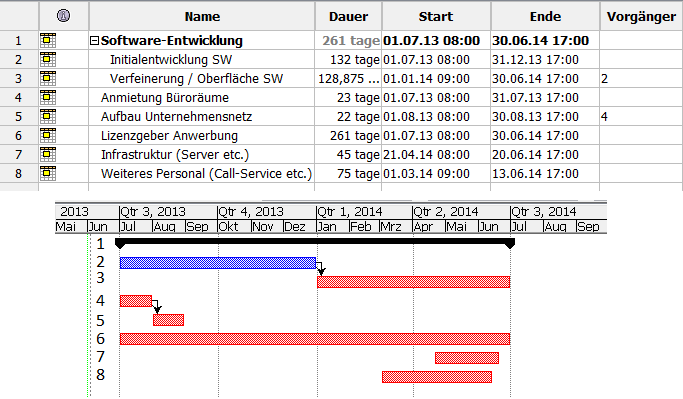
\includegraphics[scale=1.00]{zeitplan.png}
                 \caption{Zeitplan}
         \label{fig:NM}
\end{figure}

Der veranschlagte Zeitraum für diese Phase entspricht exakt einem Jahr. Er ist unterteilt in

\begin{itemize}
	\item Entwicklung der Software
	\item Infrastruktur (Firma, Ressourcen)
	\item Infrastruktur (Verträge mit Lizenzgebern)
	\item Personalmanagement
\end{itemize}

Die Entwicklung der Software ist grob unterteilt und beschäftigt sich in den ersten beiden Quartalen mit der Basis des Klienten und soll grundlegende Funktionen ermöglichen. Diese werden den Erwerb von Lizenzen, die Verwaltung dieser in Kategorien und die permanente Zugänglichkeit der Downloads umfassen. Die zweite Phase der Entwicklung wird auf Usability-Aspekte, also optimierte Oberflächen und Benutzerfreundlichkeit ausgerichtet sein. Dieser Aspekt soll natürlich auch nach dem operativen Start des Unternehmens fortgeführt werden.

Die Infrastruktur ist ebenfalls zu unterteilen. Zum einen gilt es, betriebliche Prozesse zu entwerfen und zu organisieren. Zum anderen müssen Ressourcen für den Betrieb des Unternehmens geschaffen werden, also ggf. Server, Service-Aspekte (Hotlines etc.), mögliche Bezahlsysteme (Beispiele oben genannt) und weiteres in Betracht gezogen werden. 

Für die Betreuung eines Kundenstammes in Form von Service-Leistungen, sowie für Wartung und Organisation ist eine Erweiterung des Personals geplant. Auch diese muss rechtzeitig vor Markteinstieg vollzogen sein.

\section{Strategische Ziele}

Kurzfristig steht die erfolgreiche Markteinführung mit einer ausreichend großen Auswahl von Produkten im Vordergrund. Hier muss die richtige Balance bei der Verteilung (auf die Plattform Softladen.de und den jeweiligen Anbieter der Software) von Einnahmen von Anfang an stimmen, damit längerfristig ein Erfolg dieses Formats überhaupt möglich ist. 

Mittelfristig werden sich die Ziele auf eine schnelle Reputations-Steigerung und einer damit verbundenen Marktwertsteigerung des Unternehmens beziehen. Beispielsweise soll neben Verträgen mit großen Namen der Branche eine verlässliche Plattform für kleine Entwickler geschaffen werden, die eine Verbreitung von unbekannter Software vereinfacht. Käufer haben auf diese Art eine bessere Übersicht.

Langfristig gilt es, unter den Online-Software-Vertriebsunternehmen eine Spitzenposition einzunehmen. Gegenüber anderen Unternehmen dieser Art wird das Alleinstellungsmerkmal einer Client-Software den entscheidenden Ausschlag geben, um sich in zwei Bereichen zu etablieren: Einem Stamm an Vertragspartnern, der Möglichkeiten für ein reichhaltiges Angebot an Software bietet, sowie einem breiten Feld an Kunden für die gebotenen Dienstleistungen.

Eine Erweiterung des Konzepts ist natürlich auch möglich und kann sich beispielsweise durch den Markt selber andeuten oder durch eine Ausweitung des Produktbereichs sowie neuen Funktionen ergeben.


\chapter{Produkte \& Dienstleistungen}
\section{Produkt}
Softladen.de bietet eine Rundum-Sorglos Lösung für den Einkauf von Software, die Verwaltung von Lizenzen und Installationsdateien, sowie die problemlose Integration in Arbeitsplatzrechner (Windows/Mac/Linux) durch unseren Softwareverteilungs-Client. Attraktive Software-Bundles werden dauerhaft und / oder zu Aktionen zusammengeschnürt und sind dann zu Sonderpreisen zu erwerben.\\

Kleinen und unabhängigen Softwareentwicklern, die keine Möglichkeiten einer umfassenden Vermarktung ihrer Software haben, bieten wir eine Vermarktungsplattform.\\ 

Für ausgewählte Software bieten wir zeitlich befristete Abonnements an. Dadurch können unsere Kunden hohe Anschaffungskosten für spezielle Software reduzieren. Zum Beispiel kostet eine Einzelplatzlizenz für AutoCAD LT\textcopyright 1.450,00 €. In einem Abonnement-Modell kann dieser hohe Preis für eine zeitliche befristete Nutzung deutlich reduziert werden.  \\ 

\section{Zusätzliche Dienstleistung}
Kleine und Mittelständische Unternehmen müssen sich dank unserer Lizensierungsberatung nicht mit unterschiedlichen Lizenzmodellen der unterschiedlichsten Hersteller auseinandersetzen. Anzahl und Gültigkeit der Lizenzen werden automatisch durch den Softwareverteilungs-Client geprüft.\\

Über den Client können Updates für die installierten Programme durchgeführt werden. Dabei werden die von den Herstellern zur Verfügung gestellten Updates der entsprechenden Programme genutzt. Diese Updates können automatisch oder je nach Client-Einstellungen erst nach einer Benachrichtigung, bzw. auf Anfrage des Benutzers, heruntergeladen und installiert werden. So wird eine bequeme Handhabung der Programmaktualität garantiert. Updates müssen nur ausgeführt werden sofern Kompatibilität mit anderen Programmen oder Benutzern benötigt wird. \\

Wir bieten darüber hinaus auch Beratung zu Lizensierungsfragen über ein Web-basiertes Tool, sowie im Einzelgespräch über unser Callcenter.\\ \TODO{ggf. ausschmücken}

Per e-Mail oder Telefon kann ein Kundendienst erreicht werden. Der Kundendienst dient als Ansprechpartner für Probleme bei der Kaufabwicklung. Des Weiteren kann der Kundendienst als Vermittlungsstelle bei Problemen mit der Software selbst genutzt werden und leitet die Kunden an die entsprechenden Kanäle bzw.  Kundendienste der jeweiligen Softwarehersteller weiter. \\


\chapter{Marktanalyse}
\section{Gesamtmarkt}
Die Modularität und die damit verbundenen unterschiedlichsten Einsatzbereiche schaffen
für Softladen.de eine große Breite an Marktfeldern.
\begin{itemize}
	\item Große Unternehmen
	\item Mittel bis kleine Unternehmen
	\item Private Kunden
\end{itemize}
Eine Analyse der Marktsegmente Geschäftskunde zeigt, dass es in diesen Bereichen eine große Zahl von Vergleichs- und Konkurrenzanbieter gibt. Außerdem neigen große Unternehmen dazu, Software direkt vom Hersteller zu beschaffen. Eine Markteinführung des Softladen.de in diesen Segmenten unterläge folglich einem stärkeren Konkurrenz- und Preisdruck. Aus dieser Erkenntnis heraus liegt der Geschäftsfokus im Marktsegment Privatkunde. Die Marktanalyse sowie Marketing- und Absatzplanung werden auf diesen Geschäftsbereich ausgerichtet. Weitere Geschäftsfelder, beispielsweise Mittel-bis-kleine Unternehmen, werden in diesem Geschäftsplan als Expansionsmöglichkeiten behandelt.
\section{Marktsegmentierung}
Der Markt für Softladen.de, nämlich der Softwareverkaufsmarkt ist nicht auf Deutschland beschränkt, er ist grundsätzlich weltweit dort einzuordnen, wo Software gebraucht wird. Deutschland hat im Bereich Software eine weltweit bedeutende Rolle und ist daher besonders relevant. Softladen.de soll deshalb zunächst auf Inlandskunden ausgerichtet werden. Im Zuge einer Markteinführung wird der deutschsprachige Raum Europas mit einbezogen. Zur Darstellung einer Marktübersicht Softwareanbieter werten wir Erhebung verschiedener Branchendaten dieses Marktfeldes in der Bundesrepublik Deutschland aus. Wie aus der aktuellen Erhebung der Lünendonk GmbH, Kaufbeuren (Lünendonk\textsuperscript{\textregistered}-Liste 2013\footnote[1]{\url{http://luenendonk.de/wp-content/uploads/2013/05/LUE_Liste_u_PI_2013_Standard_Software_f160520131.pdf})}, hervorgeht, haben die 25 Software-Unternehmen, die im Jahr 2012 die höchsten Umsätze in Deutschland erzielten und jeweils mehr als 60 Prozent ihres Umsatzes im Standard-Software-Geschäft machten, in Deutschland 2012 Inlandsumsätze von zusammen fast 9,4 Mrd. Euro erwirtschaftet. Das entspricht einem inländischen Marktanteil von 55 Prozent (2011: 56%).
Das Leistungsspektrum der Top 25 der Standard-Software-Branche in Deutschland konzentriert sich eindeutig auf die beiden Kernkategorien Standard-Software-Vertrieb (38%) und Software-Wartung (32%). Standard-Software-Einführung und Systemintegration machen im Durchschnitt zusammen gut 10 Prozent aus. Outsourcing, einschließlich Application Service Providing (ASP) und Software as a Service (SaaS), erreicht im Durchschnitt erst 3,8 Prozent der Umsätze. Die restlichen Anteile entfallen auf IT-Beratung (4,5%), Individual-Software-Entwicklung (3,4%), Schulung (3,6%), Hardware-Vertrieb (1,2%) und sonstige Leistungen (3,5%).
Nach Ermittlungen des Brachenverbands Bitkom stieg das Marktvolumen von Standard-AnwendungsSofware, Systemsoftware und Tools 2012 in Deutschland um 5,1 Prozent auf 17,1 Mrd. Euro (2011: 16,2 Mrd. Euro).

Trends
Aktuell entnimmt man der Presse leicht positive Trends für die Gesamtwirtschaftslage, im Besonderen für den Softwarebereich Insgesamt verkauften die vierzehn Standard-Software-Unternehmen aus der Lünendonk\textsuperscript{\textregistered}-Liste, die ihren Hauptsitz bzw. die Mehrheit ihres Grund- oder Stammkapitals in Deutschland haben, für rund 15,3 Mrd. Euro Software-Produkte an Kunden im Ausland. Daraus ergibt sich für 2012 ein Exportanteil am Gesamtumsatz dieser vierzehn Unternehmen (19,5 Mrd. Euro), der mit 78,5 Prozent die entsprechende Quote für das Vorjahr 2011 (76,1%) noch übertrifft. Ein für unser Produkt bedeutendes Ergebnis, ist der Deutscher Software-Markt in 2012 um 4,4 Prozent wächst. Für den Bereich Private Nutzung von Software erwarten Marktkenner ein überdurchschnittliches Wachstum von 20% und mehr. Die Experten berichteten zudem von dem Trend, dass Marktvolumen von SaaS weiter wächst, laut Gartner\footnote[2]{http://www.gartner.com/newsroom/id/1963815}. Beim Markteintritt von Softladen.de wird dieser Trend genutzt, indem den Firmen besondere Angebote und attraktive Preisen angeboten werden. Eine Bewertung der allgemeinen Marktdaten und der Einteilung in einzelne Segmente, führt in unserem Geschäftsbereich zum Hauptsegment Softwarelizenzverkauf und -verwaltung.

\section{Marktpotential}
Für die Quantifizierung des Marktpotentials von Softladen.de als innovativer Softwareanbieter, stehen keine relevanten Daten zur Verfügung. Die Bewertung des Marktpotentials resultiert aus der Erkenntnis, dass es ein kontinuierliches Wachstum der  Softwaremarktvolumen aber immer noch wenige effektive Plattform zur Softwarelizenzverkauf und -verwaltung in Deutschland gibt.

\textbf{Absatzmarkt}
Aus der Analyse des Datenmaterials und Befragungen potentieller Kunden entwickeln wir
Absatzzahlen für die kommenden Jahre. Dabei ist von Bedeutung, dass ein Kunde im
Durchschnitt mehr als ein Software erwerben wird. Bei den uns vorliegenden Befragungsergebnissen
geht es um die Anzahl bis zu 5 Lizenzen verschiedenster Softwares. Für unsere Absatzprognose nehmen wir an, dass jeder Kunde im Durchschnitt 1,5 Softwarelizenz abnehmen
wird.
Jahr 1:
Bestehende Anfragen nach Lieferfähigkeiten des Produktes weiterverfolgen, Vertriebsaufbau, Markteinführung
-> 500 Lizenzen
Jahr 2:
Verkauf starten, mehr Softwarehersteller im Kontakt nehmen, Referenzen zeigen, Marketing und Vertrieb auf das erforderliche Maß ausbauen
Annahme:
Kontaktaufnahme zu ca. 5000 potentiellen Kunden und 100 Softwarehersteller
-> davon ca. 1/3 Interessenten, ca. 1700 Interessenten
-> davon 10 bis 20% Kunden, die „je 1 Lizenz“ abnehmen
-> 340 Lizenzen
Jahr 3:
Vertrieb ausbauen, internationaler Vertrieb, neue Geschäftsfelder aufbauen
Annahme: 
-> Kontaktaufnahme zu ca. 10000 potentiellen Kunden
-> davon ca. 1/3 Interessenten, ca. 3500 Interessenten
-> davon 10% bis 20% Kunden, die „je 2 Lizenzen“ abnehmen
-> 1400 Lizenzen
Jahr 4:
Neben den vorgenannten Maßnahmen den Vertrieb weiter ausbauen, Erweiterung der
Produktfamilie
-> 2500 Lizenzen
Jahr 5:
Neben den vorgenannten Maßnahmen den Vertrieb weiter ausbauen.
-> 5000 Lizenzen

\textbf{Abo-Nutzung}
Neben dem Verkauf der Softwarelizenz Softladen kann das Abonutzungsmodell einen hohen Stellenwert einnehmen, da besonders Kunden an einer kurzzeitigen Nutzung interessiert sind und auf
den Kauf einer permanenten Lizenz des verzichten möchten.
In Gesprächen mit potentiellen Kooperationspartnern werden wir uns der Realisierung dieses Geschäftsfeldes annähern 

\section{Wettbewerber}
Im Hauptmarktsegment „Softwarelizenzverkauf und -verwaltung“ ist erfahrungsgemäß ein relativ hoher Anteil an Stammkunden zu erwarten, die eher bekannte Konzepte bevorzugen. Gleichzeitig sind aber viele Kunden offen gegenüber neuen Ideen. Im Bereich Softwarelizenzverkauf spielen Angebote und Preisestruktur eine sehr wichtige Rolle, d.h. der Kunde sucht nach immer neuen flexiblen Möglichkeiten, um Software kosteneffektiv zu nutzen. Für Softladen.de gibt es im Marktsegment Softwarelizenzverkauf und -verwaltung daher keine Eintrittsbarrieren. Derzeit liegt Wettbewerb nur in Teilbereichen vor. Im Zuge des Markterfolges des Softladen.de ist aber davon auszugehen, dass Wettbewerber in den Markt eintreten werden. Diese werden einerseits Hersteller von Software, andererseits möglicherweise andere Onlineplattformen mit dem Schwerpunkt Softwarelizenzverkauf und -verwaltung  sein.
Als indirekte Wettbewerber bezeichnen wir Softwareretailers, die Boxed Softwares verkaufen.


%\chapter{Markt}
%\begin{itemize}
%\item Konkurrenz (App-Stores, Softwarebilliger.de)
%\item Marktanteile
%\end{itemize}

\chapter{Vertrieb}
	\section{Vertiebskan\"ale}
	
Unser Vertriebsmodel entspricht dem Online-Direkt-Vertrieb. Ein Managementclient wird zum Download bereitgestellt, über den 
	
	Kernpunkte:\\
	\begin{itemize}
		\item Online Direkt Vertrieb
		\begin{itemize}
			\item HTTP Download
			\item Software-Management Client
				\begin{itemize}
					\item Installation
					\item Lizenzmanagement
					\item Rollenkonzept f\"ur Administration des Softwarebestandes f\"ur kleine Unternehmen
				\end{itemize}
			\item Jederzeit sofortige Lieferung
			\item Lieferzuverlässigkeit durch Elastic Cloud (Amazon S3) sichergestellt
		\end{itemize}
	\end{itemize}


\chapter{Finanzen}
  Die Eigenkapitaleinlage liegt bei 70.000 \EURcr, was 15.6\% entspricht. Diese wird zu gleichen Teilen unter den Gesellschaftern aufgeschlüsselt (10.000 \EURcr pro Gesellschafter). Im ersten Jahr wird das Programm sowie die Webseite entwickelt, ab dem zweiten Jahr werden die ersten Umsätze erschlossen.
    
    \section{Gr\"undungskosten \& Investitionen}
        Die Gründungs- und Investitionskosten belaufen sich auf 407 .780 Euro. 
        
        \begin{center}
        \begin{tabular}{|l|r|}
        \hline 
        Beschreibung & Kosten \\ 
        \hline 
        \multicolumn{2}{|l|}{\textbf{Administrative Kosten}}\\ 
        \hline 
        Anwalt/Notar & 1.000 \EURcr \\ 
        \hline 
        Marke & 300 \EURcr \\ 
        \hline 
        Gewerbe & 500 \EURcr \\ 
        \hline 
        \multicolumn{2}{|l|}{\textbf{Businessplan Kosten}} \\ 
        \hline
	      Marktanalyse & 2.400 \EURcr \\ 
        \hline
        \multicolumn{2}{|l|}{\textbf{Produktion}} \\
        \hline
	      Immobilie & 2.350 \EURcr \\ 
      	\hline
      	Maschinen & 730 \EURcr \\ 
        \hline
        \multicolumn{2}{|l|}{\textbf{Produktspezifische Kosten	}}\\
        \hline
	      Produktentwicklung & 350.000 \EURcr \\ 
      	\hline
      	\multicolumn{2}{|l|}{\textbf{Marketingkosten}}\\
      	\hline
	      Homepage & 1.000 \EURcr \\ 
      	\hline      	      	
      	\multicolumn{2}{|l|}{\textbf{Geschäftsausstattung}}\\
      	\hline
	      Telefon etc. & 1.000 \EURcr \\ 
      	\hline
      	PC & 40.000\EURcr \\ 
      	\hline
      	Drucker & 1.500 \EURcr \\ 
      	\hline
      	Büroeinrichtung & 3.000 \EURcr \\ 
      	\hline
      	\multicolumn{2}{|l|}{\textbf{Makler}}\\
      	\hline
	      Immobilienmakler & 4.000 \EURcr \\ 
      	\hline      	
      	\hline
      	\rowcolor{green}
      	\multicolumn{2}{|l|}{\textbf{Kosten bei Gründungsstart:  407.780 \EURcr}}\\ 
      	\hline
        \end{tabular} 
        \end{center}
       
     \section{Laufende Kosten}
     \section{Kapitalbedarf}
     \section{Finanzierung des Kapitalbedarfs}



%\bibliographystyle{alpha}
%\bibliography{A1}

\end{document}
